\section{Orbits and the Effective Potential}

\makelabheader %(Space for student name, etc., defined in master.tex)

\textbf{Objective}

To study classical orbits of systems like the Sun and Earth or the hydrogen atom 
to understand the physics of these orbits and the impact of angular
momentum on the shape and other properties of the orbit.

\textbf{Apparatus}

\begin{itemize}

\item {\it Excel} for plotting curves

\item {\it PhET Gravity and Orbits} simulation software$.^1$

\end{itemize}

\textbf{Overview}

Classical physics successfully describes many fundamental properties of the world
around us including the motion of the Sun, the Earth, and the denizens of our Solar System.
It also provides a starting point to study the hydrogen atom where the mathematical form of the
equations that describe the interaction of a proton and an electron (the Coulomb force)
is the same.
In this laboratory we will study the links between mechanical energy, potential energy,
and kinetic energy including the role of angular momentum in influencing 
orbits.
We will perform a simulation of the Earth-Sun system which serves as a model of
the hydrogen atom.

\textbf{Activity 1: Energy in Three Dimensions}


Consider the form of the total
mechanical energy of a light particle in three dimensions 
orbiting a much heavier one
\begin{equation}
E = \frac{1}{2} m \vec v \cdot \vec v + V(r) = 
   \frac{1}{2} m (v_x^2 + v_y^2 + v_z^2) + V(r) = 
   \frac{1}{2} m v^2 + V(r) 
\end{equation}
where $m$ is the particle's mass, $\vec v$ is its
velocity, $r=\sqrt{x^2 + y^2 + z^2}$ is the distance between Earth-Sun or electron-proton, 
and  $V(r)$ is the potential energy of the particle.
This potential depends only on the light particle's distance from the heavy one.
%We have used the definition of the momentum $\vec p = m \vec v$.
The potential energy between the electron and proton in a hydrogen atom is 
the Coulomb potential so
\begin{equation}
V_C(r) = k_e \frac{q_1 q_2}{r} =  
   - k_e \frac{e^2}{r} 
\end{equation}
where we have used the known proton and electron charges.
The potential energy between the Earth and the Sun is 
the gravitational potential so
\begin{equation}
V_G(r) = G\frac{m_1 m_2}{r} =  
   - G \frac{m_E m_S}{r} 
\end{equation}
where $G$ is the gravitational constant and $m_E$ and $m_S$ are the
mass of the Earth and Sun respectively. Note the similarity between Equations 2 and 3.

If we have an electron in the vicinity of a proton ({\it i.e.} a hydrogen atom), then
it is convenient to rewrite the kinetic energy part of Equation 1 in polar coordinates.
The proton, electron and the electron's velocity vector 
form a plane where we can describe the velocity in terms
of a radial component and an angular one
\begin{equation}
\vec v = v_r \hat r + v_t \hat \theta
\end{equation}
where $\hat r$ points radially along a line from the origin at the proton center
to the electron's position
and $\hat \theta$ is perpendicular to $\hat r$ and points so counter-clockwise rotations
are positive.

\newpage

(a) Get an expression for $v^2$ in terms of
$v_r$ and $v_t$ and substitute your result in the total energy equation (Equation 1).
Note the differences for the square of the velocity in Equation 1.
\answerspace{2.0cm}

(b) We now define the momentum associated with  the radial motion
as $\vec p_r = m\vec v_r$
and the momentum associated with the angular motion $\vec L = mr\vec v_t$.
The angular momentum $\vec L$ is a constant of the motion so it is unchanging.
Rewrite your energy equation in terms of $p_r$, $L$, $r$, and any other constants.
Include the explicit version of the Coulomb potential from Equation 2.
\answerspace{3.0cm}

(c) You should have found in part 1.b that the three-dimensional
mechanical energy of a particle in a Coulomb 
field can be written as
\begin{equation}
E = \frac{p_r^2}{2m} + \frac{L^2}{2mr^2} - k_e\frac{e^2}{r}
\end{equation}
where $L$ is a constant so the energy only depends on $r$ and $p_r$.
Make a sketch of the potential energy as a function of $r$.
What are the limiting values of the potential?
\answerspace{3.0cm}

(d) The angular momentum $L$ is a constant of the motion so the last two terms in 
Equation 5 can be treated as a single `effective' potential $V_{eff}$ that governs the radial motion
of particles.
Make a sketch of those last two terms added together as a function of $r$ for constant $L$.
How is your figure different from the one in 1.c?
\answerspace{3.0cm}


(e) Since the energy is constant you can draw it on your previous sketch as a flat, straight
line. We are considering bound states (the hydrogen atom) so $E < 0$.
Draw an energy line for a bound state on your previous sketch.
Does your energy `curve' intersect the effective potential curve anywhere?
For a classical particle like a ball rolling on a hill or a satellite orbiting the
Earth,
what happens at this intersection?
Describe the motion of a classical particle in this potential.
What restrictions are there on the energy $E$ of a classical particle?
\answerspace{3.0cm}

\textbf{Activity 2: Plotting the Energy}

(a) To visualize the motion of the Earth around the Sun or a classical electron around
a proton we will plot combinations of the components of the total energy in Equation 5
using {\it Excel}. To start, generate a column of values of the radial distance between
the two particles.
In the top cell of Column A enter `$r$' to label the column.
In the second cell of the column type in {\tt =ROW()/10} and hit enter.
You should see a number appear in the cell.
This is the value of `$r$'.
Click on the small square in the lower, right corner of the cell and drag down the 
column until you have eighty values in the column.

(b) In the top cell of the adjacent column (Column B) 
enter `{\tt 7.6/r\^{}2}' to label the column and then calculate 
$7.6/r^2$ using the values of $r$ from Column A you just created.
You might enter {\tt =7.6/(A2*A2)}.
Click and drag down that new cell to match all the entries in Column A.
The constants here are chosen for the hydrogen atom so the radius $r$
is in angstroms ($10^{-10}~m$) and the energies are in electron-Volts ($eV$).

(c) Go to the top cell of the next column to the right (Column C), enter `{\tt -14.4/r}' to label
the column and calculate $-14.4/r$ for all the values of $r$ in Column A.

(d) Go to the top cell of the next column (you're now on the fourth column, Column D),
enter `{\tt Veff}' to label it, and calculate
the sum of the calculations in the previous two columns.

(e) Now make charts in {\it Excel} of the three functions of $r$ you generated above.
Put all of the curves on a single plot for comparison.
To do this highlight all the data you have generated in Columns A-D 
including the labels at the top
of each column and go to 
{\tt Insert $\rightarrow$ Chart $\rightarrow$ Scatter(X,Y) Chart}.
You should immediately get a plot with $r$ on the horizontal axis and the three
curves you just calculated along with a legend defining each curve.
To make the plot easier to interpret zoom in on 
the central region of the plot by right-clicking on the vertical axis labels 
and select {\tt Format Axis}. Under {\tt Axis Options} change the minimum and 
maximum {\tt Bounds} to $-8$ and $+2$, respectively. Print the plot and attach it to this unit.

(f) We can now investigate what these curves mean. Use a ruler to draw a
straight, horizontal line at an energy value of $-3.4~eV$ on your plot.
We are considering bound states (the hydrogen atom or the Earth orbiting the Sun) 
so $E < 0$.
You can think of this straight line as representing the value of the total 
mechanical energy. See Equation 5.

(g) Does your total energy `curve' intersect the effective potential curve $V_{eff}$ anywhere?
If not, consult your instructor.
For a classical particle like a ball rolling on a hill or a satellite orbiting the
Earth, what happens at this intersection?
What is the radial part of the kinetic energy  at this point
(the first term on the right-hand-side of Equation 5)?
Describe the motion of a classical particle (the Earth orbiting the Sun or an
electron orbiting a proton) in this potential with this value of the total mechanical
energy.

\answerspace{3.0cm}

(h) Draw a dashed, straight, horizontal line at a value of $-7.5~ eV$ on your plot. This means the
total energy is less than the efffective potential energy.
What does that imply about the radial part of the kinetic energy?
See Equation 5.
Does this make sense?
What restrictions are there on the energy $E$ of a classical particle?

\answerspace{2.5cm}

\textbf{Activity 3: Simulating Orbits}

We will now use a simulation of the Earth-Sun system as a surrogate for the
hydrogen atom. We can do this because the form of the Coulomb force is
mathematically the same as the gravitational force.

(a) Obtain the {\it Gravity and Orbits} simulation at the address below

\url{https://phet.colorado.edu/sims/html/gravity-and-orbits/latest/gravity-and-orbits_en.html}

and start it up. Select the {\tt Models} option and then configure the
software using the checkboxes on the right-hand-side of the tabletop.
See the figure below for the options to pick.

\begin{figure}[htb!]
\begin{center}
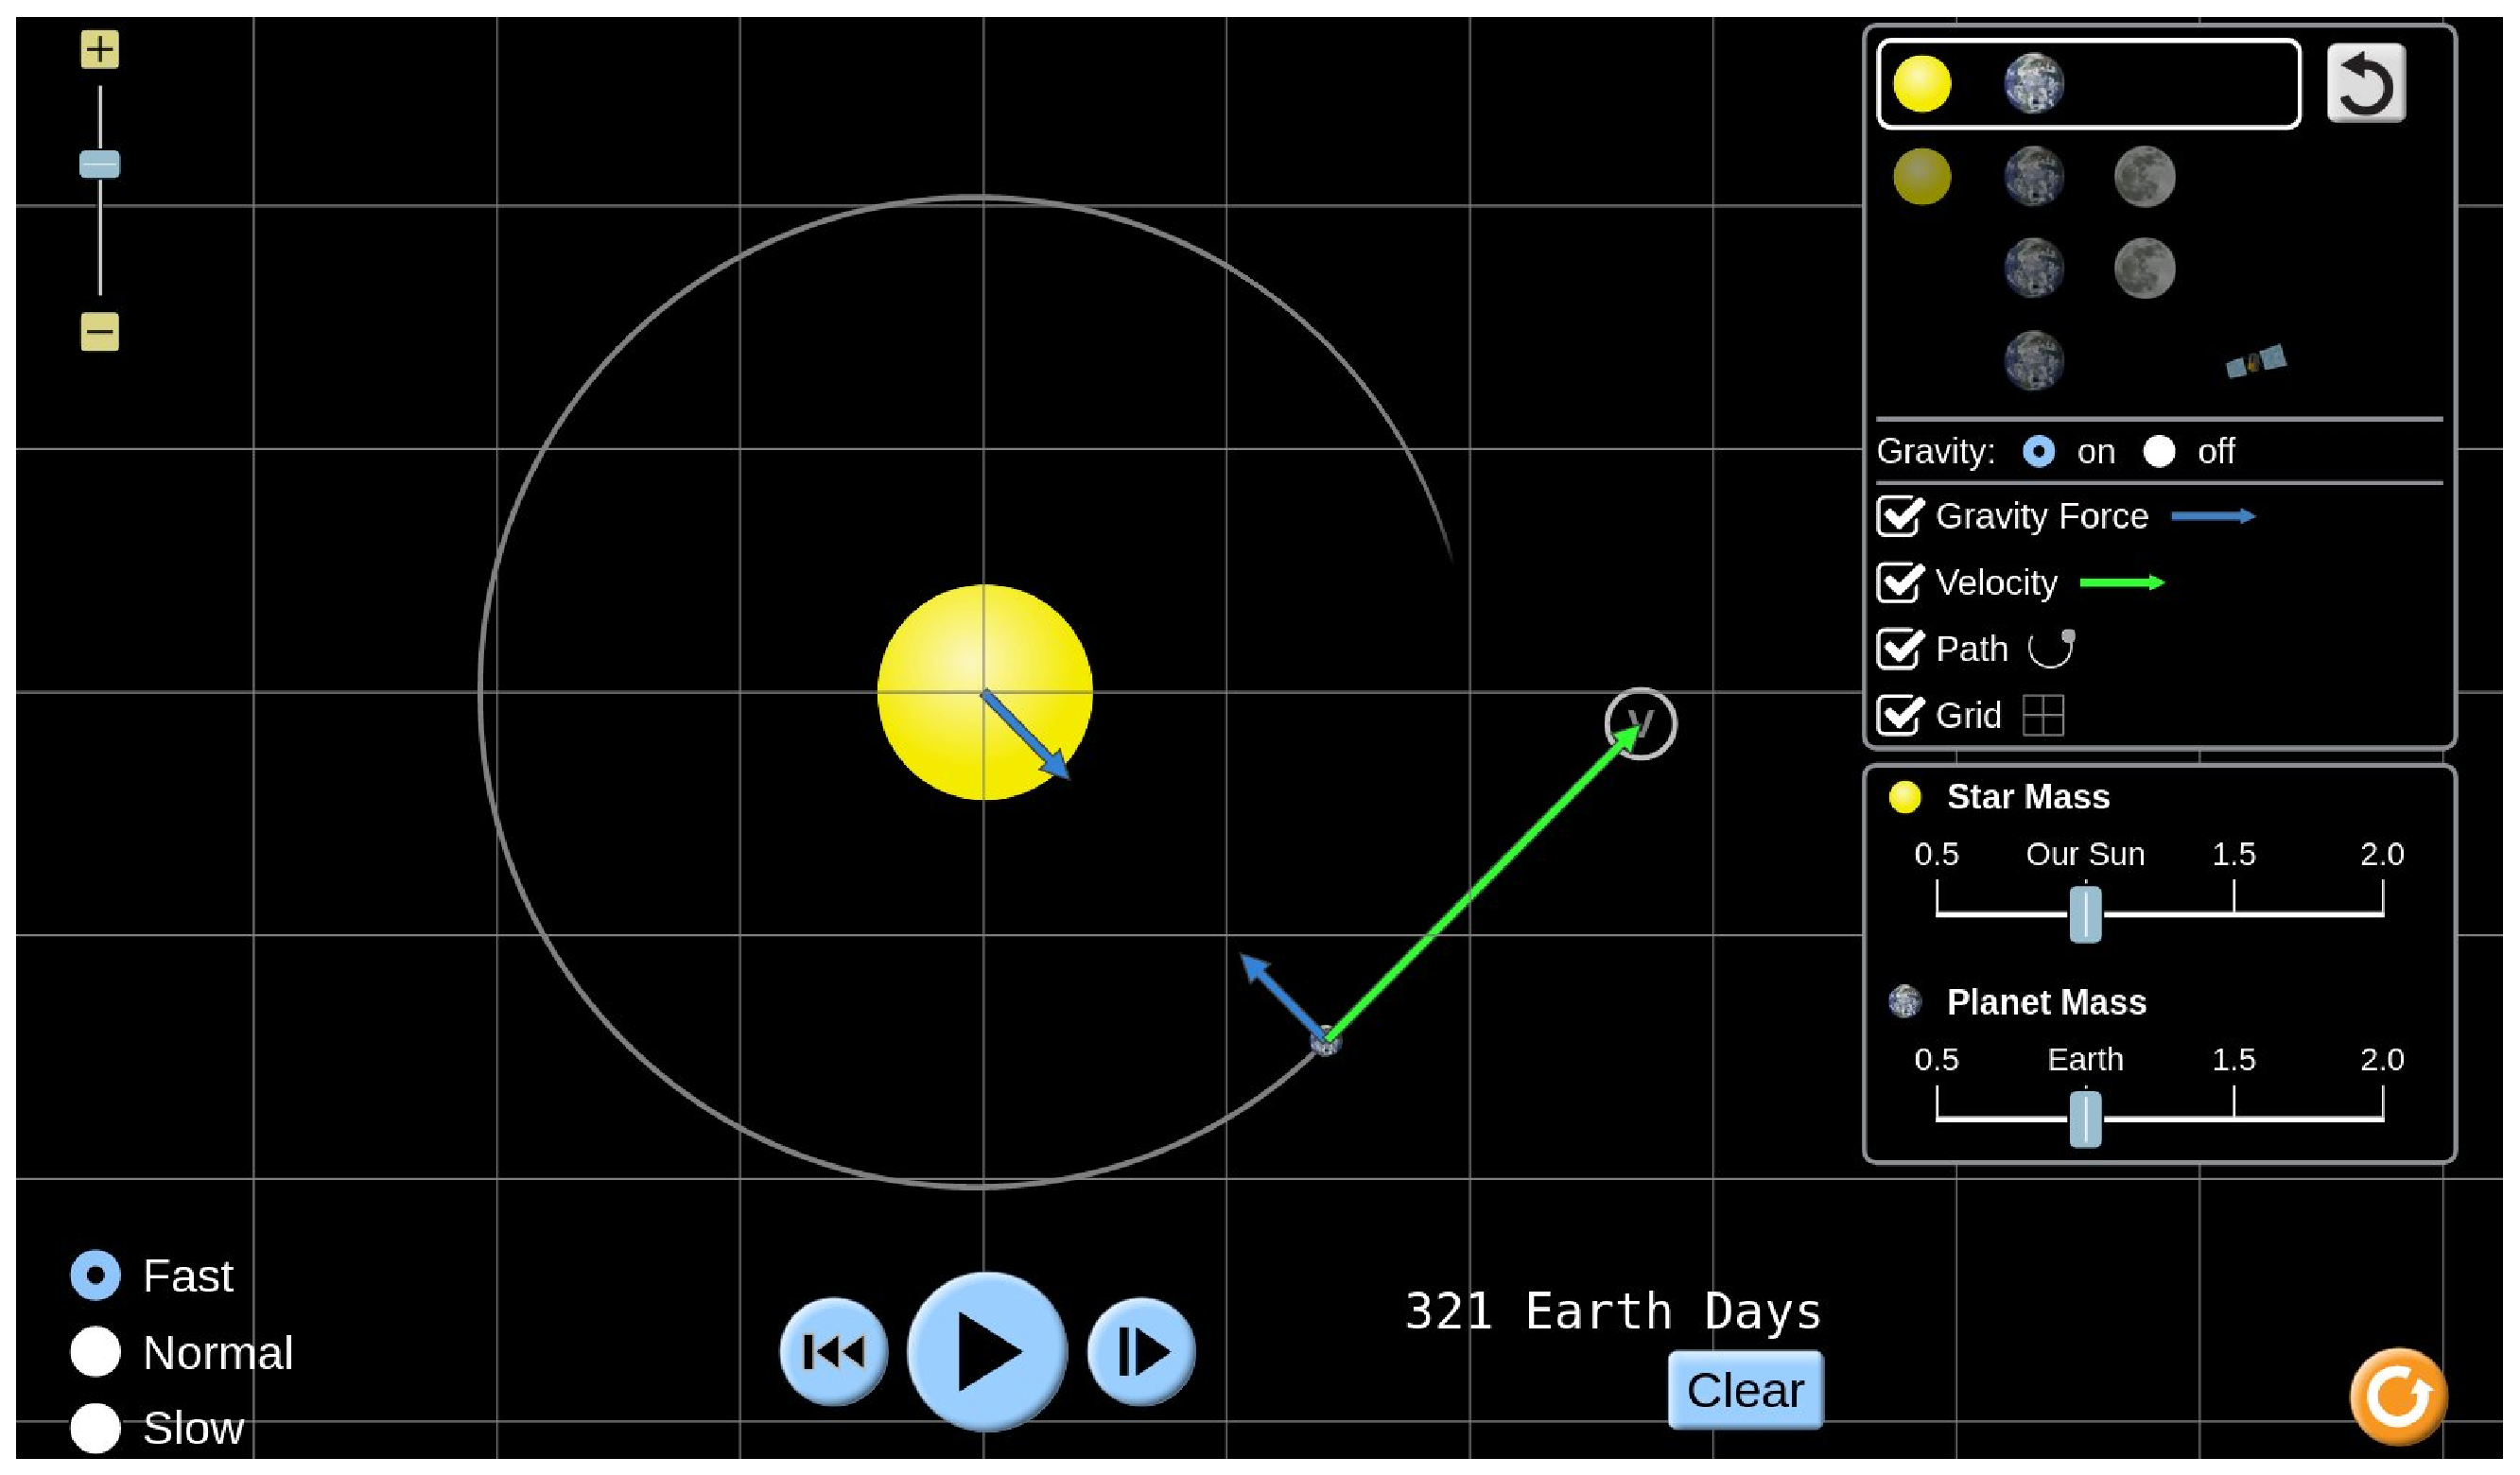
\includegraphics[height=2.75in]{classicalOrbits/phetClassicalOrbits2.eps}
\caption{Tabletop of {\it Gravity and Orbits} simulation from PhET.}
\end{center}
\end{figure}

(b) The green vector attached to the Earth shows the velocity and moves with the 
Earth.  The initial configuration of the Earth is motion in a circle.
Is there any component of the Earth's velocity in the radial direction?
Can you draw any conclusions about the value of the first term in Equation 5.
Recall your figure of the different components of the mechanical energy in Activity 2.
If the Earth is moving in a circle where would you draw the horizontal line representing
the total mechanical energy on your plot?
Make that drawing.

\answerspace{2.0cm}

(c) Without changing anything in the simulation what do you predict would happen to the Earth's
trajectory if  you increased its velocity?
Would the radius of the circular orbit increase?
Explain your choice.

\answerspace{2.0cm}

(d) Stop the simulation. Increase the length of the green velocity vector 
without changing its direction by clicking on the arrowhead 
and dragging it to increase its length.
Restart the simulation.
You can change the overall scale of the tabletop by moving the slide
in the upper, left-hand corner.
Is the orbit still a circle?
Is the first term in Equation 5 (the radial part of the kinetic energy) constant?
What happens to the length of the year, {\it i.e} the time for one full orbit?

\answerspace{2.5cm}

(e) Stop the simulation. Rotate the Earth's green velocity vector about $30^\circ $ inward.
How does the orbit change? 
Where is the Earth's speed largest?
Where is the Earth's speed smallest?
Explain your observations using the conservation of mechanical energy.
What happens to the length of the year, {\it i.e} the time for one full orbit?

\answerspace{2.5cm}
 
\noindent {\bf References}

\begin{enumerate}

\item PhET Interactive Simulations, University of Colorado Boulder, \url{http://phet.colorado.edu},
last accessed April 16, 2021.

\end{enumerate}
